\documentclass[sigconf]{acmart}


\IfFileExists{upquote.sty}{\usepackage{upquote}}{}
\IfFileExists{microtype.sty}{% use microtype if available
  \usepackage[]{microtype}
  \UseMicrotypeSet[protrusion]{basicmath} % disable protrusion for tt fonts
}{}
\makeatletter
\@ifundefined{KOMAClassName}{% if non-KOMA class
  \IfFileExists{parskip.sty}{%
    \usepackage{parskip}
  }{% else
    \setlength{\parindent}{0pt}
    \setlength{\parskip}{6pt plus 2pt minus 1pt}}
}{% if KOMA class
  \KOMAoptions{parskip=half}}
\makeatother

%%
%% This is file `sample-manuscript.tex',
%% generated with the docstrip utility.
%%
%% The original source files were:
%%
%% samples.dtx  (with options: `manuscript')
%% 
%% IMPORTANT NOTICE:
%% 
%% For the copyright see the source file.
%% 
%% Any modified versions of this file must be renamed
%% with new filenames distinct from sample-manuscript.tex.
%% 
%% For distribution of the original source see the terms
%% for copying and modification in the file samples.dtx.
%% 
%% This generated file may be distributed as long as the
%% original source files, as listed above, are part of the
%% same distribution. (The sources need not necessarily be
%% in the same archive or directory.)
%%
%%
%% Commands for TeXCount
%TC:macro \cite [option:text,text]
%TC:macro \citep [option:text,text]
%TC:macro \citet [option:text,text]
%TC:envir table 0 1
%TC:envir table* 0 1
%TC:envir tabular [ignore] word
%TC:envir displaymath 0 word
%TC:envir math 0 word
%TC:envir comment 0 0
%%
%%
%% The first command in your LaTeX source must be the \documentclass command.


% Options for packages loaded elsewhere
\PassOptionsToPackage{unicode}{hyperref}
\PassOptionsToPackage{hyphens}{url}
\PassOptionsToPackage{dvipsnames,svgnames,x11names}{xcolor}

\IfFileExists{bookmark.sty}{\usepackage{bookmark}}{\usepackage{hyperref}}

%% PANDOC PREAMBLE BEGINS


\providecommand{\tightlist}{%
  \setlength{\itemsep}{0pt}\setlength{\parskip}{0pt}}\usepackage{longtable,booktabs,array}
\usepackage{calc} % for calculating minipage widths
% Correct order of tables after \paragraph or \subparagraph
\usepackage{etoolbox}
\makeatletter
\patchcmd\longtable{\par}{\if@noskipsec\mbox{}\fi\par}{}{}
\makeatother
% Allow footnotes in longtable head/foot
\IfFileExists{footnotehyper.sty}{\usepackage{footnotehyper}}{\usepackage{footnote}}
\makesavenoteenv{longtable}
\usepackage{graphicx}
\makeatletter
\def\maxwidth{\ifdim\Gin@nat@width>\linewidth\linewidth\else\Gin@nat@width\fi}
\def\maxheight{\ifdim\Gin@nat@height>\textheight\textheight\else\Gin@nat@height\fi}
\makeatother
% Scale images if necessary, so that they will not overflow the page
% margins by default, and it is still possible to overwrite the defaults
% using explicit options in \includegraphics[width, height, ...]{}
\setkeys{Gin}{width=\maxwidth,height=\maxheight,keepaspectratio}
% Set default figure placement to htbp
\makeatletter
\def\fps@figure{htbp}
\makeatother

% !TEX program = xelatex
\definecolor{mypink}{RGB}{219, 48, 122}
\makeatletter
\makeatother
\makeatletter
\makeatother
\makeatletter
\@ifpackageloaded{caption}{}{\usepackage{caption}}
\AtBeginDocument{%
\ifdefined\contentsname
  \renewcommand*\contentsname{Table of contents}
\else
  \newcommand\contentsname{Table of contents}
\fi
\ifdefined\listfigurename
  \renewcommand*\listfigurename{List of Figures}
\else
  \newcommand\listfigurename{List of Figures}
\fi
\ifdefined\listtablename
  \renewcommand*\listtablename{List of Tables}
\else
  \newcommand\listtablename{List of Tables}
\fi
\ifdefined\figurename
  \renewcommand*\figurename{Figure}
\else
  \newcommand\figurename{Figure}
\fi
\ifdefined\tablename
  \renewcommand*\tablename{Table}
\else
  \newcommand\tablename{Table}
\fi
}
\@ifpackageloaded{float}{}{\usepackage{float}}
\floatstyle{ruled}
\@ifundefined{c@chapter}{\newfloat{codelisting}{h}{lop}}{\newfloat{codelisting}{h}{lop}[chapter]}
\floatname{codelisting}{Listing}
\newcommand*\listoflistings{\listof{codelisting}{List of Listings}}
\makeatother
\makeatletter
\@ifpackageloaded{caption}{}{\usepackage{caption}}
\@ifpackageloaded{subcaption}{}{\usepackage{subcaption}}
\makeatother
\makeatletter
\makeatother
%% PANDOC PREAMBLE ENDS

\setlength{\parindent}{10pt}
\setlength{\parskip}{0pt}

\hypersetup{
  pdftitle={Coding Non-Visually in Visual Studio Code: Collaboration Towards Accessible Development Environment for Blind Programmers},
  pdfauthor={JooYoung Seo; Megan Rogge},
  colorlinks=true,
  linkcolor={blue},
  filecolor={Maroon},
  citecolor={Blue},
  urlcolor={red},
  pdfcreator={LaTeX via pandoc, via quarto}}

%% \BibTeX command to typeset BibTeX logo in the docs
\AtBeginDocument{%
  \providecommand\BibTeX{{%
    Bib\TeX}}}

%% Rights management information.  This information is sent to you
%% when you complete the rights form.  These commands have SAMPLE
%% values in them; it is your responsibility as an author to replace
%% the commands and values with those provided to you when you
%% complete the rights form.
\setcopyright{acmcopyright}
\copyrightyear{2018}
\acmYear{2018}
\acmDOI{XXXXXXX.XXXXXXX}

%% These commands are for a PROCEEDINGS abstract or paper.
\acmConference[ASSETS]{The 25th International ACM SIGACCESS Conference
on Computers and Accessibility}{October 22--25, 2023}{New York, NY}
\acmPrice{15.00}
\acmISBN{978-1-4503-XXXX-X/18/06}

%% Submission ID.
%% Use this when submitting an article to a sponsored event. You'll
%% receive a unique submission ID from the organizers
%% of the event, and this ID should be used as the parameter to this command.
%%\acmSubmissionID{123-A56-BU3}

%%
%% For managing citations, it is recommended to use bibliography
%% files in BibTeX format.
%%
%% You can then either use BibTeX with the ACM-Reference-Format style,
%% or BibLaTeX with the acmnumeric or acmauthoryear sytles, that include
%% support for advanced citation of software artefact from the
%% biblatex-software package, also separately available on CTAN.
%%
%% Look at the sample-*-biblatex.tex files for templates showcasing
%% the biblatex styles.
%%

%%
%% The majority of ACM publications use numbered citations and
%% references.  The command \citestyle{authoryear} switches to the
%% "author year" style.
%%
%% If you are preparing content for an event
%% sponsored by ACM SIGGRAPH, you must use the "author year" style of
%% citations and references.
%% Uncommenting
%% the next command will enable that style.
%%\citestyle{acmauthoryear}


%% end of the preamble, start of the body of the document source.
\begin{document}


%%
%% The "title" command has an optional parameter,
%% allowing the author to define a "short title" to be used in page headers.
\title[VSCode\_A11y]{Coding Non-Visually in Visual Studio Code:
Collaboration Towards Accessible Development Environment for Blind
Programmers}

%%
%% The "author" command and its associated commands are used to define
%% the authors and their affiliations.
%% Of note is the shared affiliation of the first two authors, and the
%% "authornote" and "authornotemark" commands
%% used to denote shared contribution to the research.


  \author{JooYoung Seo}
  \orcid{0000-0002-4064-6012}
            \affiliation{%
                  \institution{School of Information Sciences,
University of Illinois at Urbana-Champaign}
                          \streetaddress{614 E Daniel St}
                          \city{Champaign}
                                  \country{USA}
                          \postcode{61820}
              }
        \author{Megan Rogge}
  
            \affiliation{%
                  \institution{Microsoft}
                          \streetaddress{1 Microsoft Way}
                          \city{Redmond}
                                  \country{USA}
                          \postcode{98052}
              }
      
\renewcommand{\shortauthors}{Seo and Rogge}

%% By default, the full list of authors will be used in the page
%% headers. Often, this list is too long, and will overlap
%% other information printed in the page headers. This command allows
%% the author to define a more concise list
%% of authors' names for this purpose.
%\renewcommand{\shortauthors}{Trovato et al.}
%%  
%% The abstract is a short summary of the work to be presented in the
%% article.
\begin{abstract}
This paper delineates a fruitful collaboration between blind and sighted
developers, aiming to augment the accessibility of Visual Studio Code
(VSCode). Our shared journey is portrayed through examples drawn from
our interaction with GitHub issues, pull requests, review processes, and
insider's releases, each contributing to an improved VSCode experience
for blind developers. One key milestone of our co-design process is the
establishment of an accessible terminal buffer, a significant
enhancement for blind developers using VSCode. Other innovative outcomes
include Git Diff audio cues, adaptable verbosity settings, intuitive
help menus, and a targeted accessibility testing initiative. These
tailored improvements not only uplift the accessibility standards of
VSCode but also provide a valuable blueprint for open-source developers
at large. Through our shared dedication to promoting inclusivity in
software development, we aim for the strategies and successes shared in
this paper to inspire and guide the open-source community towards
crafting more accessible software environments.    
\end{abstract}

%%
%% The code below is generated by the tool at http://dl.acm.org/ccs.cfm.
%% Please copy and paste the code instead of the example below.
%%
\begin{CCSXML}
<ccs2012>
  <concept>
      <concept_id>10003120.10011738.10011774</concept_id>
      <concept_desc>Human-centered computing~Accessibility design and evaluation methods</concept_desc>
      <concept_significance>500</concept_significance>
      </concept>
</ccs2012>
\end{CCSXML}

\ccsdesc[500]{Human-centered computing~Accessibility design and evaluation methods}

%%
%% Keywords. The author(s) should pick words that accurately describe
%% the work being presented. Separate the keywords with commas.
\keywords{nonvisual programming, accessibility, integrated development
environment, visual studio code}


%%
%% This command processes the author and affiliation and title
%% information and builds the first part of the formatted document.
\maketitle

\setlength{\parskip}{-0.1pt}

\hypertarget{introduction}{%
\section{Introduction}\label{introduction}}

An integrated development environment (IDE) is an application that
conveniently provides essential functions for the entire programming
process, including source editing, compiling and interpreting, and
debugging. IDEs have become an essential tool for not only software
developers but also STEM engineers and data scientists in many fields to
efficiently manage their computing environments
\citep{altharBuildingIntelligentIntegrated2021, crossJGRASPIntegratedDevelopment2007, janssenPyironIntegratedDevelopment2019}.
However, blind developers\footnote{We use the identity-first language
  (i.e., blind people) instead of the person-first language (i.e.,
  people with visual impairments or vision loss) when addressing this
  population, guided by the perspective of the National Federation of
  the Blind.} are not able to take advantage of the many features that
graphical user interface (GUI)-based IDEs offer
\citep{potluriCodeTalkImprovingProgramming2018}. For example, syntax
highlighting, code autocompletion and autosuggestion, diagnostics and
linting, variable watches and breakpoints are underutilized even among
experienced blind programmers, and many blind developers are still
working manually with simple text like Notepad, along with runtime and
compile terminals
\citep{mealinExploratoryStudyBlind2012, albusaysElicitingProgrammingChallenges2016, albusaysInterviewsObservationBlind2017}.
Behind this problem are intertwined issues of accessibility and
learnability. Because different IDEs use different architectures and
have different levels of accessibility compliance, blind developers face
a new learning curve each time they use an IDE. Blind developers also
face the additional challenge of learning the non-visual workaround of
accessing an IDE with a screen reader
\citep{mealinExploratoryStudyBlind2012}. Although there is a community
of blind programmers called Program-L
\citep{johnsonProgramLOnlineHelp2022} where blind programmers help and
support each other, IDEs remain a daunting barrier for blind people.

These difficulties are a major socio-technical barrier to blind
developers reaching their full potential in the computing field and to
social and professional participation. From the perspective of the
social model \citep{oliverSocialModelDisability2013}, which recognizes
that an individual's disability may stem from structures and cultures
that sociotechnically limit their access rather than from physical,
sensory, cognitive, or emotional issues, we can see that IDE
accessibility issues are no longer a group-specific problem that blind
people must endure, but a collective task for the technology community
to reduce barriers together. Specifically, to address these issues,
blind and sighted developers need to work together to understand the
challenges that blind developers face in using IDEs and then
collaboratively find ways to address those challenges. This perspective
is consistent with the ``interdependent framework''
\citep{bennettInterdependenceFrameAssistive2018, degreefInterdependentVariablesRemotely2021}
that other accessibility researchers have advocated to move away from
the dependency of accessibility on the individual with disabilities and
instead view accessibility as a shared responsibility of people with and
without disabilities and the environment surrounding them.

This paper is the empirical product of blind and sighted developers who
have thought deeply about these issues and actively collaborated. We
describe how the first author, who is blind, and the second author, who
is sighted, have been working together to make the open source IDE
Visual Studio Code (VSCode) non-visually accessible and what specific
accessibility features have been implemented as a result of our
collaboration. In the following sections, we start with some background
on how our collaboration began, then present our methods and
deliverables. Finally, we'll share some insights from our collaboration.

\hypertarget{sec-vscode_a11y}{%
\section{Background: Visual Studio Code and
Accessibility}\label{sec-vscode_a11y}}

Visual Studio Code is a lightweight, free, and powerful open-source code
editor\footnote{In this paper, the terms integrated development
  environment and code editor are used interchangeably.} which runs on
the desktop and on the web. It is available for Windows, macOS, and
Linux. It has built-in support for JavaScript, TypeScript, and Node.js
and a rich ecosystem of extensions for other languages and runtimes,
such as C++, C\#, Java, Python, PHP, Go, .NET, and more. Accessibility
has been a core priority for VSCode since its inception. Among the many
architectural elements of VSCode, the following, in particular, has
contributed to its accessibility. First, VSCode is a cross-platform
application built with the Chromium-based Electron Framework. In other
words, VSCode is an application built using web technologies, which
gives it the flexibility to follow web accessibility guidelines and
respond to the accessibility of various screen readers and assistive
technologies regardless of the operating system. Second, Monaco, the
primary editor of VSCode, has its own screen reader compatibility mode,
which is designed to be selectively turned on and off depending on the
user's intent. Third, Microsoft's xterm.js terminal, used by VSCode,
also provides a separate screen reader accessibility switch in
accordance with the Web Accessibility Guidelines. Finally, VSCode is an
open-source project where anyone can suggest and fix features on GitHub,
and a daily insiders version is built so that real users can quickly use
the alpha version and provide feedback to the developers, which in turn
leads to a higher quality, user-centered stable version.

The accessibility benefits of VSCode and tips on how to take advantage
of them have been shared among members of the Program-L mailing list, a
community of blind programmers. In addition, due to its growing
popularity among blind programmers, there has been a recent spate of
research and development of accessible plug-ins based on VSCode
\citep{potluriCodeWalkFacilitatingShared2022, stogerDesigningInclusiveAccessible2022}.
Nevertheless, the fact that VSCode is accessible compared to other IDEs
does not necessarily mean that it is easy for blind programmers to use.
For example, there is still a constant stream of questions on Program-L
about VSCode, not only about its basic usage, but also about features
that have already been made accessible in VSCode, such as the terminal,
debugging, and the Jupyter Notebook extension, which suggests that many
blind programmers are often frustrated by the tricky usability of VSCode
accessibility. The following section describes how the authors of this
paper collaborated to address this usability issue of VSCode
accessibility.

\hypertarget{methods}{%
\section{Methods}\label{methods}}

\hypertarget{author-profiles-and-collaboration-context}{%
\subsection{Author Profiles and Collaboration
Context}\label{author-profiles-and-collaboration-context}}

The first author of this paper is blind with only light perception,
currently working as an assistant professor in the School of Information
Sciences at the University of Illinois at Urbana-Champaign. At the
university, he teaches introductory data science courses using R and
Python to undergraduate and graduate students. As a lifelong non-visual
programmer, he has experience with a variety of IDEs, including Visual
Studio, Eclipse, and Net Bean, and text editors such as Emacs/Emacspeak,
VIM, and NotePad++, on Linux, Mac, and Windows operating systems, using
a variety of screen readers (e.g., JAWS, NVDA, Narrator, VoiceOver, and
Orca) and refreshable braille displays. He is a certified professional
in accessibility core competencies (CPACC) from the International
Association of Accessibility Professionals and has contributed code to a
number of open-source data science projects to improve screen reader
accessibility, including RStudio IDE Server and the web-based data
science dashboard Shiny, reproducible technical publishing systems
(e.g., R Markdown, bookdown, and Quarto), and the data table package gt.
He is also a member of Program-L. In this community, he has experienced
first-hand the challenges that blind programmers face in using IDEs and
how they overcome them by interacting with other blind programmers and
participating in discussions. To improve these community-wide
challenges, he created his first issue on the Microsoft VSCode public
GitHub site on May 31, 2020, and has since created a total of 164
contributions (87 issues; 76 post comments and mentions; 1 pull request)
to actively suggest usability improvements for blind programmers in
VSCode and interact with other open source developers\footnote{see
  online appendix at https://github.com/jooyoungseo/assets2023\_vscode}.

The second author is a VSCode software engineer. She has worked on the
product since graduating from the University of North Carolina at Chapel
Hill in 2020 with the highest distinction and highest honors for her
research and work with Dr.~Gary Bishop on semi-automated gaming for
users with a wide range of disabilities. About 10 months ago, Megan
requested to take over responsibility for the product's accessibility.
Since then, she has been working closely with JooYoung and the community
to understand accessibility issues and collaborate on solutions.

\hypertarget{co-design-and-expert-review}{%
\subsection{Co-Design and Expert
Review}\label{co-design-and-expert-review}}

Our collaborative approach utilized the strategies of co-design and
expert review. The co-design methodology fosters a joint creation
process between the user and developer, enabling the developer to grasp
the user's requirements and, in turn, develop a product aligning with
these needs \citep{sandersCocreationNewLandscapes2008}. In this
framework, JooYoung acted as an expert, given his multi-faceted role as
a daily VSCode user, an experienced open-source contributor, a data
science educator, and an accessibility professional. He outlined his
varied computing experiences to Megan and swiftly assessed his
accessibility patches. Our communication began asynchronously via
GitHub, debating on issues and potential solutions. Following a few
weeks of this pattern, we mutually agreed that scheduled meetings could
prove more efficient and productive. JooYoung's wealth of ideas and
insights complemented Megan's eagerness to learn and her drive to
enhance the product's accessibility. In these sessions, JooYoung
demonstrated his use of VS Code by sharing his screen on Zoom, posing
queries, and suggesting alterations. Conversely, Megan provided her
insights, questioned various aspects, and noted down bugs or features
requiring attention. These exchanges facilitated Megan's understanding
of JooYoung's usage of VS Code and enabled JooYoung to comprehend the
product components, which could otherwise remain confusing or
undiscovered.

Despite the implementation of regular meetings, asynchronous
communication via GitHub and email persisted. Megan regularly composed
follow-up emails encapsulating their meeting discoveries prior to
circulating them to the entire VSCode team. JooYoung further scrutinized
these issues, providing comments if anything was overlooked or during
the fix-testing process.

\hypertarget{co-designed-deliverables}{%
\section{Co-Designed Deliverables}\label{co-designed-deliverables}}

While nearly all VS Code accessibility fixes and features within the
past year are products of this collaboration, below are several of the
highlights.

\hypertarget{terminal-buffer}{%
\subsection{Terminal Buffer}\label{terminal-buffer}}

As discussed in Section~\ref{sec-vscode_a11y}, xterm.js, the terminal UI
utilized by VSCode, incorporates a screen-reader accessibility mode for
blind people. However, a discernible gap emerged between accessibility
(the ability to access information) and usability (the convenience of
use), which led to recurring concerns among blind programmers.

Consider the following scenario: you type and execute the command
\texttt{echo\ hello;\ echo\ world;} in the terminal. You will observe
\texttt{hello} and \texttt{world} as two separate lines of output. The
existing accessibility mode of xterm.js presented this content through a
screen reader using an aria-live alert and permitted a line-by-line
review of the terminal output history with the \texttt{Ctrl+UpArrow} and
\texttt{Ctrl+DownArrow} keys. This worked well for short and simple
outputs, but for lengthy outputs with intricate error messages or
computational results, a swift speech-to-text message was insufficient
for capturing substantial information in human working memory.

An additional concern is that \texttt{Ctrl+Up/DownArrow} navigation
keys, designed to review terminal history, delivered the entire contents
of the focused line to the screen reader as a single object. This made a
detailed examination of terminal contents on a character or word basis
challenging. Blind users had to switch the reading mode using the screen
reader's virtual cursor (i.e., browse mode in NVDA; QuickNav mode in
VoiceOver) to review the terminal content more thoroughly. To resume
terminal input, they had to disable the virtual cursor and return to
forms mode (focus mode in NVDA; QuickNav off in VoiceOver), leading to
significant inconvenience.

JooYoung initiated a discussion on the official Microsoft VSCode GitHub
page, bringing attention to these issues and proposing solutions (see
\href{https://github.com/microsoft/vscode/issues/98918}{microsoft/vscode\#98918:
Terminal output div container should be more accessible for screen
readers}). Megan, meanwhile, developed terminal shell integration, a
feature allowing VS Code to comprehend terminal activities, facilitating
user-friendly command navigation, command output copying, and more.
JooYoung demonstrated that the terminal buffer remained inaccessible for
screen reader users, as it didn't support arrow key navigation. He
proposed that the output view's accessible experience be integrated into
the terminal. Upon discussing with a colleague, Megan incorporated the
same underlying component into the terminal, making the previously
inaccessible terminal buffer navigable via arrow keys for blind users.
More specifically, he suggested replacing the terminal output with a
text editor buffer supporting standard arrow-key navigation. The
implementation, requiring over a year of technical experimentation and
collaborative testing, yielded fruitful results. Initial efforts to
redirect the terminal output web container, designated as ``list'', to
aria ``document'' or ``textbox'' landmarks proved unsatisfactory due to
varying screen reader and platform support levels for aria. The terminal
output was then converted into a text area with ``contenteditable'' and
``read only'' attributes, which also did not gel with the screen
reader's speech buffer. Eventually, we created a separate accessible
terminal buffer by transferring the terminal output to VSCode's native
Monaco editor, ensuring optimal accessibility and usability for all
blind users on all platforms and screen readers. This feature,
well-received by many blind users in the Program-L community, was
officially introduced in the VSCode stable version 1.75.

In Figure 1, a screenshot depicts the terminal accessible buffer in
action. A screen reader is shown focusing on an error message from a
task terminal and audibly announcing: ``{[}watch-client {]}
{[}12:41:01{]} Error: /Users/meganrogge/Repos/\newline
vscode/vscode/src/vs/workbench/contrib/accessibility/brow\newline
ser/accessibilityContributions.ts(198,63): `)' expected.''. Users can
navigate the displayed content using standard arrow keys without having
to switch between different navigation modes.

\begin{figure}
{\centering 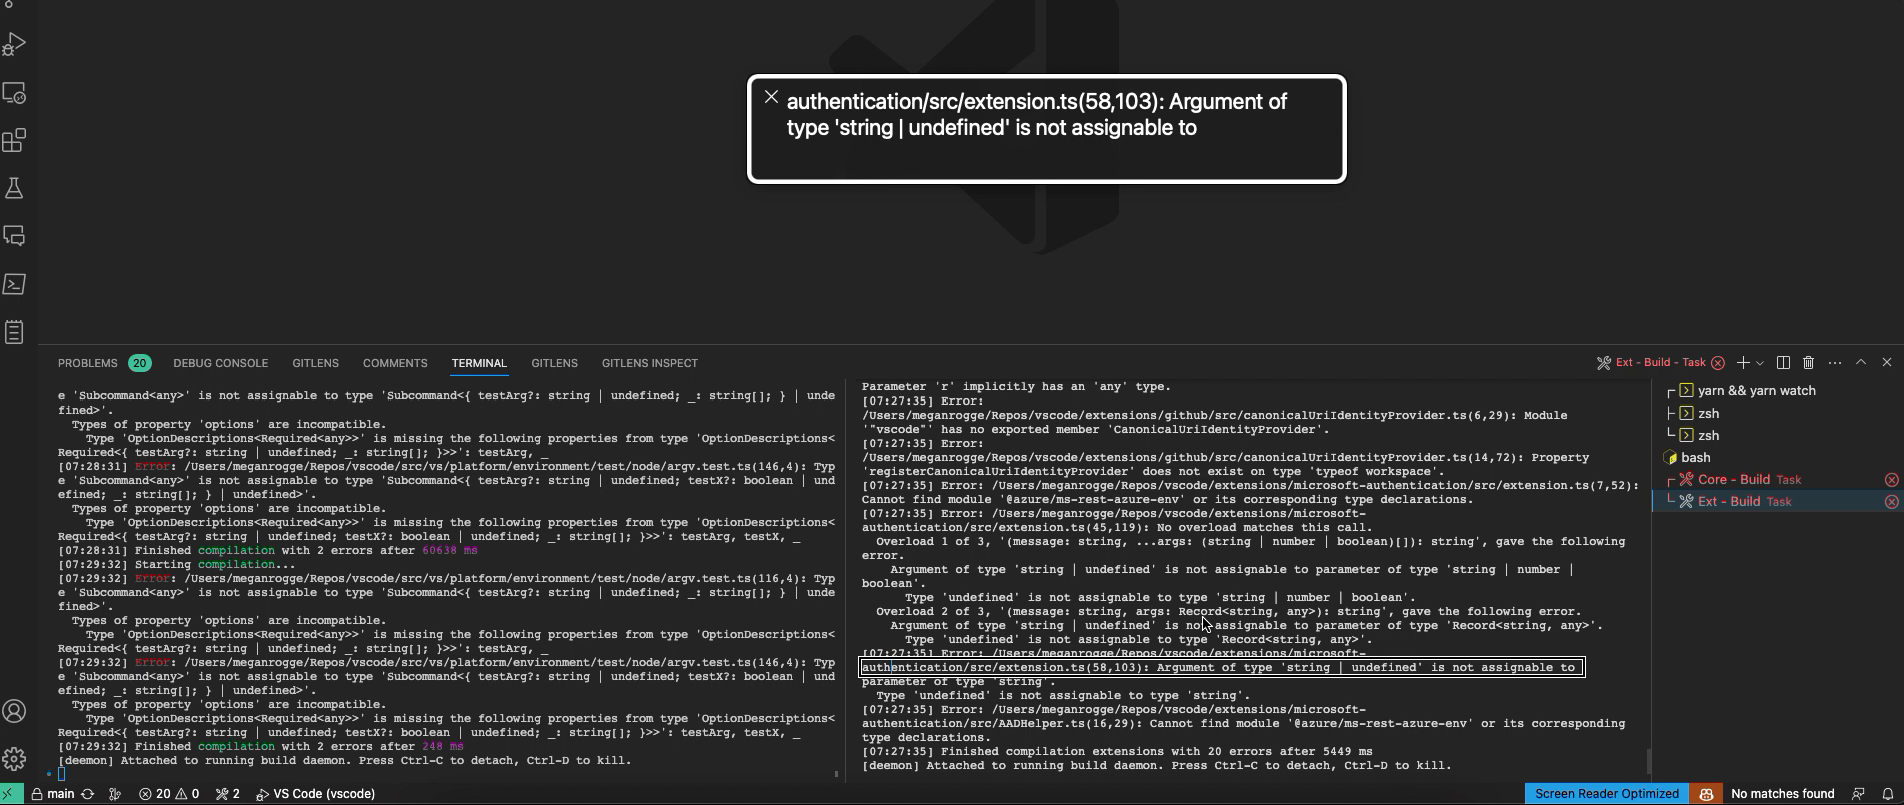
\includegraphics{images/terminal-accessible-buffer.png}}
\caption{The terminal accessible buffer.}
\Description{The terminal accessible buffer.}
\end{figure}

\hypertarget{git-diff-and-audio-cues}{%
\subsection{Git Diff and Audio Cues}\label{git-diff-and-audio-cues}}

Git has been around for decades as a version control tool like SVN, but
its popularity has really taken off with the rise of open-source social
coding platforms based on Git, such as GitHub and GitLab. Naturally,
there have been many personal and social needs for blind people to
utilize Git in collaborative environments. Git is originally a
Unix-based command-line tool, so in terms of accessibility, blind people
can use a screen reader to fully utilize Git in a terminal. However,
since Git has over 100 core Git commands, and the number of possible
combinations could be in the millions, using Git via the command line
takes a lot of effort and time to become proficient. In response,
various tools have emerged that allow users to utilize Git as a GUI, and
VSCode is a very popular IDE that supports a collaborative environment
using Git.

Git's \texttt{git\ diff} feature enables users to track changes and
compare differences between files or commits in an asynchronous
collaborative setting. Using this command, new additions are marked in
green with a \texttt{+} prefix, while deletions appear in red with a
\texttt{-} prefix. VSCode ensured that the \texttt{git\ diff} feature is
accessible to screen reader users. When users had the desired files or
commits open for comparison, they could quickly navigate to the
differences using the \texttt{F7} key (Go to Next Difference) and
\texttt{Shift+F7} (Go to Previous Difference). These differences were
prefixed with a \texttt{+} or \texttt{-} sign to denote additions or
deletions, respectively. Of course, this approach was fine from an
accessibility standpoint, but there was room for improvement in terms of
usability and convenience for blind users. For example, visual
affordances like color coding and \texttt{+-} signs in
\texttt{git\ diff} allowed sighted people to skim quickly, but blind
people had to listen to additional speech prefixes, pronounced + (plus)
and - (dash), serially and wait for information before each change.
Furthermore, depending on the punctuation pronunciation settings of the
screen reader, the +- sign could be omitted to the screen reader.

To ameliorate this, JooYoung suggested adding non-visual, non-speech,
and audible affordances to \texttt{git\ diff} in addition to \texttt{+-}
signs, so that blind people can hear and understand them easily (see
\href{https://github.com/microsoft/vscode/issues/147226}{microsoft/vscode\#147226}).
Audio cues, often referred to as ``earcons'', are non-speech sound
effects that enhance accessibility. While VSCode and Microsoft's Visual
Studio have only recently started supporting them, their importance in
non-visual programming was highlighted decades ago by TV Raman, a blind
computer scientist. He introduced the concept of earcons as a
counterpart to visual icons when he developed Emacspeak
\citep{ramanEmacspeakSpeechInterface1996}. For example, audio cues allow
the editor to quickly recognize if the current line of code contains an
error or a warning, instead of just saying ``error'' or ``warning''
verbally, the editor will read out the unique sound associated with the
error or warning. These sounds can also be delivered in parallel with
text-to-speech information from a screen reader, allowing blind
programmers to quickly perceive the context of the code, similar to the
benefits of quickly scanning code with different color coding for those
who receive visual feedback on code with their eyes. JooYoung had
several Zoom meetings with Megan and Amnon Freidlin (Microsoft's sound
designer), and through an iterative process, finalized the three audio
cues used in the \texttt{git\ diff} context. These were the diff line
Inserted sound, which is heard when something new is added (\texttt{+}),
the diff line Deleted sound, which is heard when something existing is
removed (\texttt{-}), and the diff line Modified sound, which is heard
when something existing is modified (\texttt{+-}, \texttt{-+}). Our
success came with some trial and error. For example, an early problem
was that the Diff Line Inserted and Diff Line Deleted sounds had a
similar range and texture, making it difficult to distinguish between
them. JooYoung realized that this was a common complaint in Program-L
beyond his personal experience, so he worked with the sound designer to
test and finalize a sample file that was as self-explanatory as possible
and didn't interfere with the sound of the screen reader speech. Of
course, we had to leave the potential issue of the static audio cues we
chose not being able to adequately accommodate users with hearing
impairments in certain ranges as a future work in progress, but this
feature greatly improved the usability of our non-visual programming.

\hypertarget{verbosity-settings-and-help-menus}{%
\subsection{Verbosity Settings and Help
Menus}\label{verbosity-settings-and-help-menus}}

JooYoung created issues pointing out places where minor tweaks to the
order or content of an aria-label could yield massive productivity
improvements for screen reader users. Megan fixed some such instances
and pointed team members toward others, providing guidance about best
practices going forward. Megan started self-hosting with a screen reader
shortly after this in order to proactively identify other problems. She
felt overwhelmed by the noise and noticed some content was repeated ad
nauseum, so created an issue and sought the feedback of JooYoung, who
suggested that screen reader verbosity settings remedy this and a
similar approach could be applied to VS Code's aria content.
Additionally, JooYoung shared that while it was helpful to meet and
learn about the new features via our meetings, most screen reader users
did not have this luxury. Megan and her colleague, Daniel, brainstormed
about a discoverable way for screen reader users to find out about
terminal features. Upon terminal focus, an aria-label conveyed how to
access the terminal's accessibility help menu. To reduce noise, this
hint could be disabled with a verbosity setting. Since then, help menus
and verbosity settings have been added for the Copilot inline and panel
chat, notebook, and other features. For example, the terminal
accessibility help menu contains important information for screen reader
users such as commands to run like ``Run Recent Command (Ctrl+R)''
(Figure 2). A screen reader user can use arrow keys to read the content
line by line, character by character.

\begin{figure}
{\centering 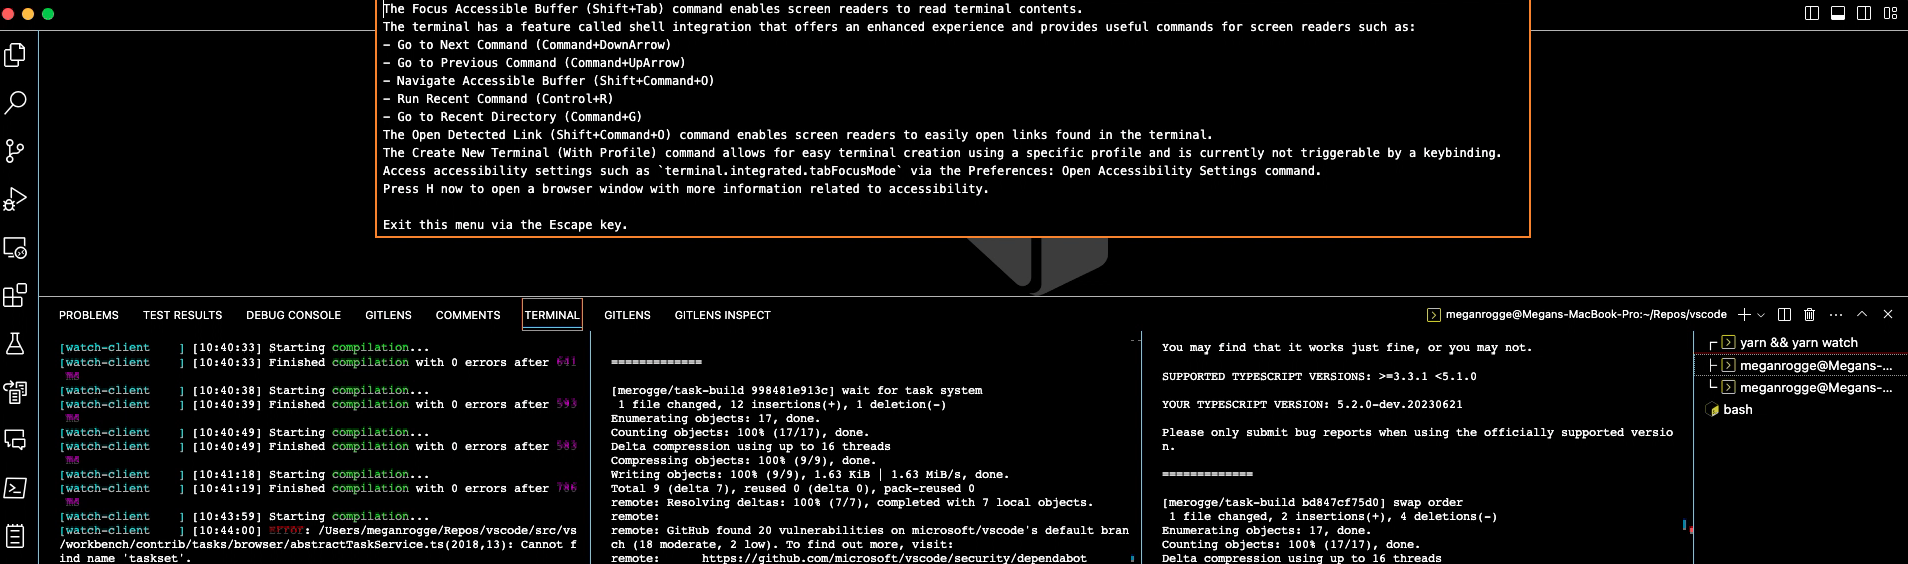
\includegraphics{images/terminal-help-menu.png}}
\caption{The terminal help menu}
\Description{The terminal help menu}
\end{figure}

\hypertarget{accessibility-testing-initiative}{%
\subsection{Accessibility Testing
Initiative}\label{accessibility-testing-initiative}}

JooYoung consistently provided feedback on GitHub, highlighting issues
with both old and new features in VS Code. His active engagement and
insights were pivotal in spotlighting an overlooked area. Megan, a key
accessibility member of the VSCode team, noticed that despite testing
new features on every platform - MacOS, Linux, and Windows at the end of
each month before a release, the screen reader experience had been
neglected. Inspired by JooYoung's observations, Megan advocated for a
new protocol: after a feature is released, it will be tested with screen
readers in the next iteration. Additionally, she initiated retroactive
tests on features to rectify this historical oversight.

\hypertarget{discussion-and-conclusion}{%
\section{Discussion and Conclusion}\label{discussion-and-conclusion}}

In our collaborative journey, blending the expertise of both sighted and
blind developers, we've unearthed pivotal insights about open-source
accessibility. Our endeavors with Visual Studio Code serve as a case in
point. Megan and JooYoung's
\href{https://learn.microsoft.com/en-us/events/vs-code-day-2023/accessibilty-in-vs-code}{livestream
seminar} accentuated the profound impact of merging accessibility
considerations with open-source development.

Open-source platforms are foundational in the tech realm. Our reach and
influence cascade into multiple offshoot applications. Hence, embedding
accessibility in these parent projects can have a magnified effect,
promoting inclusivity across numerous derivative platforms. The
participatory nature of open-source projects, welcoming feedback from a
diverse array of users, is both a strength and a challenge. JooYoung's
collaboration, while external to Microsoft, highlights this open
engagement. Yet, a pertinent concern is the potential marginalization of
voices unfamiliar with platforms like GitHub. For open-source teams,
this underscores the necessity to proactively engage with and seek
feedback from these underrepresented communities. Such engagement is not
just about hearing, but understanding and integrating feedback. The
synergy between Megan and JooYoung exemplifies the potential outcomes
when such engagements are cultivated. A recurring theme from our
experience is the importance of proactive accessibility considerations.
Post-design modifications often present challenges, emphasizing the need
for early integration of accessibility measures. Drawing these threads
together, our co-design experience underscores the imperative of
fostering an inclusive ethos in open-source development. By ensuring a
platform that is receptive to diverse voices, we can move closer to a
universally accessible coding ecosystem.

\begin{acks}
We extend our gratitude to Program-L, an online community of blind
programmers, for their invaluable feedback and testing of VS Code, as
well as their insightful accessibility suggestions. We also appreciate
the VS Code team for their commitment to accessibility. Special thanks
to Isidor Nikolic, Kai Maetzel, and Daniel Imms for their dedication and
invaluable insights; to Raymond Zhao and Roberto Perez for enhancing the
site's accessibility; to José Vilmar Estácio de Souza, Amnon Freidlin,
Marie Robbins, and Gino Scarpino for their diligent testing and
collaboration.
\end{acks}

\bibliographystyle{ACM-Reference-Format}
\bibliography{bibliography.bib}

%% begin pandoc before-bib
%% end pandoc before-bib
%% begin pandoc biblio
%% end pandoc biblio
%% begin pandoc include-after
%% end pandoc include-after
%% begin pandoc after-body
%% end pandoc after-body

\end{document}
\endinput
%%
%% End of file `sample-manuscript.tex'.
